\documentclass[12pt]{article}

\usepackage[a4paper,margin=1in]{geometry}
\usepackage{amsmath,amssymb}
\usepackage{newtxtext,newtxmath} % Times-style font
\usepackage{fancyhdr}
\usepackage{listings}
\usepackage{graphicx}
\usepackage{float}
\usepackage{algorithm}
\usepackage{algpseudocode}
\usepackage{booktabs}
\usepackage{xcolor}

\setlength{\textfloatsep}{10pt}
\setlength{\floatsep}{10pt}

\setlength{\parindent}{0pt}
\setlength{\parskip}{5pt}

% Keep entire document at 12 pt
\AtBeginDocument{
    \fontsize{12pt}{14pt}\selectfont
}

\lstdefinestyle{code}{
    language=Python,
    basicstyle=\ttfamily\fontsize{9.5pt}{11.5pt}\selectfont,
    breaklines=true,
    breakatwhitespace=false,
    frame=single,
    numbers=left,
    numberstyle=\tiny\color{gray},
    keywordstyle=\color{blue},
    commentstyle=\color{gray},
    stringstyle=\color{green!50!black},
    columns=fullflexible,
    keepspaces=true,
    showstringspaces=false
}

\lstdefinestyle{output}{
    basicstyle=\ttfamily\fontsize{9pt}{11pt}\selectfont,
    breaklines=true,
    breakatwhitespace=false,
    frame=single,
    numbers=none,
    backgroundcolor=\color{gray!6},
    columns=fullflexible,
    keepspaces=true,
    showstringspaces=false
}

% ------------------------------------------------
% Header
% ------------------------------------------------

\pagestyle{fancy}
\fancyhf{}

\fancyhead[L]{Name: Kishan Sahu{\hspace{4cm}}}
\fancyhead[R]{Enrollment No.: P26DS017{\hspace{3.5cm}}}

\renewcommand{\headrulewidth}{0.4pt}
\setlength{\headheight}{15pt}

% ------------------------------------------------
% Code formatting
% ------------------------------------------------

\lstset{
    basicstyle=\ttfamily\fontsize{9.5pt}{11.5pt}\selectfont,
    breaklines=true,
    frame=single,
    columns=fullflexible,
    keepspaces=true,
    showstringspaces=false
}

\begin{document}

% ------------------------------------------------
% TITLE
% ------------------------------------------------

\begin{center}
\textbf{Computer Science and Engineering Department, SVNIT, Surat}\\
\textbf{M.Tech. I -- Semester I}\\
\textbf{Machine Learning (CSDS105)}\\
\textbf{Lab Assignment 6: Comprehensive Study of Text and Feature Normalization in Machine Learning}
\end{center}

\vspace{0.3cm}

\section{Introduction and Problem Formulation}

In applied machine learning for Natural Language Processing (NLP), \textbf{normalization} is universally cited as an indispensable prerequisite. However, the term ``normalization'' is fundamentally overloaded, spanning two structurally distinct hierarchies:
\begin{enumerate}
    \item \textbf{Linguistic / Text-Level Normalization}: Morphological standardization converting unstructured characters and tokens into canonical root forms (case folding, punctuation stripping, stopword pruning, stemming, and lemmatization).
    \item \textbf{Mathematical / Feature-Level Normalization}: Coordinate transformations scaling numerical vector representations across document rows (e.g., $L_1$ and $L_2$ normalization) or across feature columns (e.g., Min-Max, MaxAbs, and Standard $Z$-score scaling).
\end{enumerate}

A pervasive misconception in empirical NLP is that applying feature scalers unconditionally improves classifier performance. In reality, diverse machine learning algorithms—ranging from probabilistic generative estimators (Naive Bayes) and instance-based metric learners (K-Nearest Neighbors) to non-parametric tree ensembles (Decision Trees) and linear hyperplanes (Perceptrons)—exhibit radically conflicting mathematical sensitivities to normalization. This experimental laboratory provides a rigorous benchmarking of these interactions using the canonical \textbf{SMS Spam Collection} dataset.

\subsection{Dataset Description and Exploratory Analysis}
The experimental corpus is the public Kaggle SMS Spam Collection dataset comprising $N = 5,572$ mobile SMS messages partitioned into legitimate communications (\texttt{ham}) and fraudulent promotions (\texttt{spam}).

Key empirical characteristics of the dataset:
\begin{itemize}
    \item \textbf{Class Imbalance}: The dataset is heavily skewed, containing $4,825$ \texttt{ham} instances ($86.60\%$) and $747$ \texttt{spam} instances ($13.40\%$).
    \item \textbf{Message Length Disparity}: Legitimate \texttt{ham} messages exhibit a concise median length of $\sim 52$ characters, whereas unsolicited \texttt{spam} messages are characteristically verbose (median length of $\sim 149$ characters) to maximize advertising payload.
\end{itemize}

\begin{figure}[H]
    \centering
    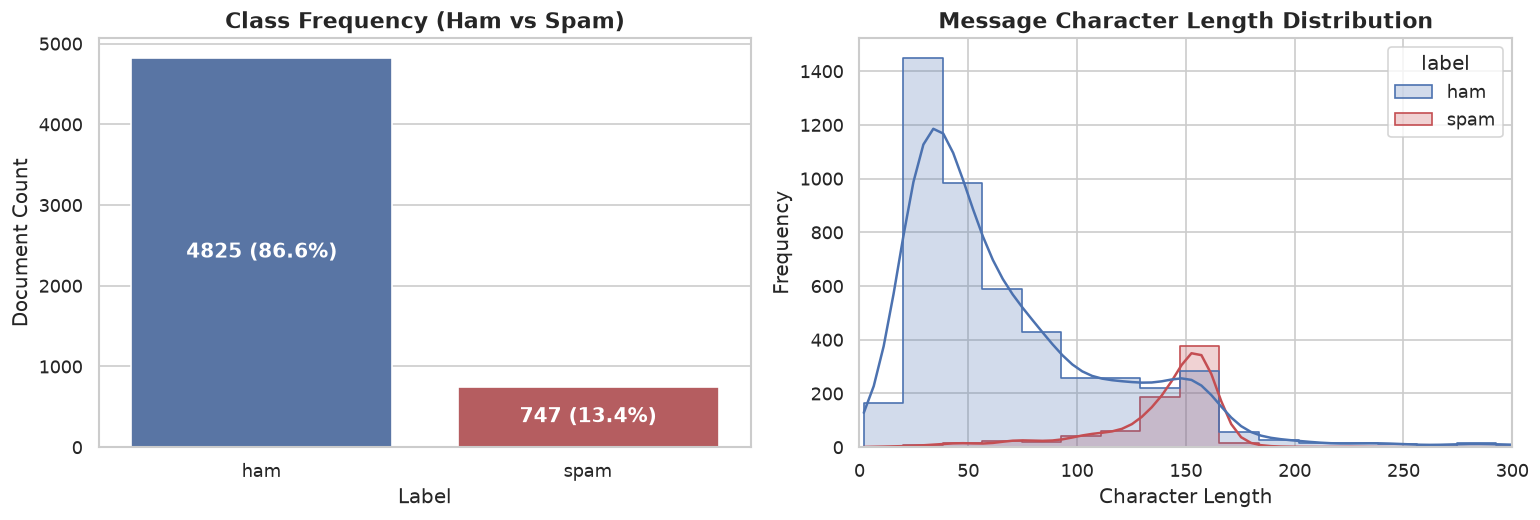
\includegraphics[width=0.92\textwidth]{figures/class_and_length_distributions.png}
    \caption{Exploratory Data Analysis: (Left) Class frequency showing dominant ham distribution; (Right) Kernel density estimation (KDE) and histogram of message character lengths demonstrating distinct multimodal length distributions between ham and spam.}
    \label{fig:distributions}
\end{figure}

\section{Theoretical Foundations: Normalization Taxonomy}

\subsection{Level 1: Linguistic Text-Level Normalization}
Text normalization reduces vocabulary cardinality by mapping morphological variations of a token to a unified canonical base:
\begin{itemize}
    \item \textbf{Case Folding and Regex Filtering}: Maps all characters to lowercase and strips non-alphanumeric punctuation:
    \begin{equation}
        s_{\text{clean}} = \text{regex\_replace}(s_{\text{lower}}, \text{[}\text{\textasciicircum a-z0-9}\text{]}, \text{` '})
    \end{equation}
    \item \textbf{Stopword Elimination}: Filters high-frequency functional syntax words (e.g., ``the'', ``is'', ``at'') carrying negligible domain discriminability:
    \begin{equation}
        \mathcal{V}_{\text{pruned}} = \{w \in \mathcal{V} \mid w \notin \mathcal{S}_{\text{stopwords}}\}
    \end{equation}
    \item \textbf{Morphological Reduction (Stemming vs. Lemmatization)}:
    \begin{itemize}
        \item \textit{Porter Stemming}: A rule-based heuristic chopping affixes (e.g., ``running'', ``runs'' $\to$ ``run''; ``studies'' $\to$ ``studi'').
        \item \textit{WordNet Lemmatization}: A lexical vocabulary lookup utilizing morphological analysis to return true dictionary base forms (lemmas).
    \end{itemize}
\end{itemize}

\subsection{Level 2: Numerical Feature-Level Normalization}
Let $\mathbf{X} \in \mathbb{R}^{N \times D}$ denote the document-term frequency matrix, where row $\mathbf{x}_i = [x_{i,1}, x_{i,2}, \dots, x_{i,D}]$ represents document $i$ across vocabulary size $D$.

\subsubsection{1. Row-Wise Vector Normalization (Document-Level)}
Row-wise operations normalize each document vector independently along its feature dimensions:
\begin{itemize}
    \item \textbf{$L_1$ Norm (Taxicab / Manhattan Normalization)}:
    Scales the vector such that feature values sum to unity ($1.0$), transforming counts into a discrete empirical probability distribution over terms:
    \begin{equation}
        \|\mathbf{x}_i\|_1 = \sum_{j=1}^{D} |x_{i,j}|, \quad \mathbf{x}_{i}^{(L_1)} = \frac{\mathbf{x}_i}{\|\mathbf{x}_i\|_1}
    \end{equation}
    \item \textbf{$L_2$ Norm (Euclidean / Unit Sphere Normalization)}:
    Projects each document vector onto a unit hypersphere ($\|\mathbf{x}_{i}^{(L_2)}\|_2 = 1.0$):
    \begin{equation}
        \|\mathbf{x}_i\|_2 = \sqrt{\sum_{j=1}^{D} x_{i,j}^2}, \quad \mathbf{x}_{i}^{(L_2)} = \frac{\mathbf{x}_i}{\|\mathbf{x}_i\|_2}
    \end{equation}
    \textbf{Geometric Implication}: Given two $L_2$-normalized vectors $\mathbf{u}$ and $\mathbf{v}$, their squared Euclidean distance directly reduces to a monotonic linear function of \textbf{Cosine Similarity}:
    \begin{equation}
        \|\mathbf{u} - \mathbf{v}\|_2^2 = \|\mathbf{u}\|_2^2 + \|\mathbf{v}\|_2^2 - 2(\mathbf{u} \cdot \mathbf{v}) = 1 + 1 - 2\cos(\theta) = 2(1 - \cos(\theta))
    \end{equation}
    Thus, $L_2$ normalization eliminates document length distortion for distance-based estimators.
\end{itemize}

\subsubsection{2. Column-Wise Feature Scaling (Corpus-Level)}
Column-wise operations normalize each word dimension $j \in \{1, \dots, D\}$ across all $N$ corpus instances:
\begin{itemize}
    \item \textbf{MaxAbs Scaling}: Scales by the absolute maximum observed count per feature without centering:
    \begin{equation}
        x_{i,j}' = \frac{x_{i,j}}{\max_{k} |x_{k,j}|} \in [0, 1]
    \end{equation}
    Preserves matrix sparsity while constraining magnitude.
    \item \textbf{Min-Max Scaling}: Scales features bounded within $[0, 1]$:
    \begin{equation}
        x_{i,j}' = \frac{x_{i,j} - \min_{k} x_{k,j}}{\max_{k} x_{k,j} - \min_{k} x_{k,j}}
    \end{equation}
    \item \textbf{Standard Scaling ($Z$-Score Normalization)}: Enforces zero empirical mean and unit variance:
    \begin{equation}
        z_{i,j} = \frac{x_{i,j} - \mu_j}{\sigma_j}, \quad \text{where } \mu_j = \frac{1}{N}\sum_{k=1}^N x_{k,j}, \quad \sigma_j = \sqrt{\frac{1}{N}\sum_{k=1}^N (x_{k,j} - \mu_j)^2}
    \end{equation}
    \textbf{Critical Consequence}: Centering subtracts the mean $\mu_j > 0$ from zero entries, converting sparse matrices into dense structures and introducing negative values that violate multinomial frequency models.
\end{itemize}

\newpage
\section{Experimental Setup and Pipeline Implementation}

\subsection{Environment Setup and Ingestion}
The implementation utilizes Scikit-Learn for vectorization and estimators, NLTK for linguistics, and Pandas/NumPy for matrix manipulation.

\begin{lstlisting}[style=code]
# 1. Imports and Environmental Configuration
import os
import re
import warnings
import urllib.request
import numpy as np
import pandas as pd
import matplotlib.pyplot as plt
import seaborn as sns

# NLTK for text-level normalization
import nltk
from nltk.corpus import stopwords
from nltk.stem import WordNetLemmatizer, PorterStemmer

# Scikit-Learn for vectorization, scaling, models, and evaluation
from sklearn.model_selection import train_test_split
from sklearn.feature_extraction.text import CountVectorizer
from sklearn.preprocessing import normalize, MaxAbsScaler, MinMaxScaler, StandardScaler
from sklearn.neighbors import KNeighborsClassifier
from sklearn.naive_bayes import MultinomialNB, ComplementNB
from sklearn.tree import DecisionTreeClassifier
from sklearn.linear_model import Perceptron
from sklearn.metrics import accuracy_score, precision_score, recall_score, f1_score, confusion_matrix

warnings.filterwarnings('ignore')
print("Environment and libraries loaded successfully.")
\end{lstlisting}

\begin{lstlisting}[style=output]
Environment and libraries loaded successfully.
\end{lstlisting}

\subsection{Dataset Ingestion and Preprocessing Utilities}
The corpus is ingested and cleaned using custom regex tokenization, stopword removal, and WordNet lemmatization.

\begin{lstlisting}[style=code]
# Ingest SMS Spam Collection Dataset
data_dir = 'data'
os.makedirs(data_dir, exist_ok=True)
data_file = os.path.join(data_dir, 'sms_spam_collection.tsv')

if not os.path.exists(data_file):
    print("Downloading SMS Spam dataset from public Kaggle mirror...")
    url = "https://raw.githubusercontent.com/justmarkham/DAT8/master/data/sms.tsv"
    urllib.request.urlretrieve(url, data_file)
    print("Download complete.")
else:
    print(f"Dataset found locally at '{data_file}'.")

df = pd.read_csv(
    data_file,
    sep='\t',
    header=None,
    names=['label', 'text']
)
df['target'] = df['label'].map({'ham': 0, 'spam': 1})
print(f"Total instances: {len(df)}")
print(f"Class Distribution:\n{df['label'].value_counts()}")

# Implement Text Normalization Utilities
nltk.download('stopwords', quiet=True)
nltk.download('wordnet', quiet=True)
nltk.download('omw-1.4', quiet=True)

stop_words = set(stopwords.words('english'))
lemmatizer = WordNetLemmatizer()
stemmer = PorterStemmer()

def normalize_text(text, use_stemming=False):
    text = text.lower()
    text = re.sub(r'[^a-z0-9\s]', ' ', text)
    tokens = text.split()
    tokens = [t for t in tokens if t not in stop_words and len(t) > 1]
    if use_stemming:
        tokens = [stemmer.stem(t) for t in tokens]
    else:
        tokens = [lemmatizer.lemmatize(t) for t in tokens]
    return ' '.join(tokens)

df['clean_text'] = df['text'].apply(normalize_text)
\end{lstlisting}

\begin{lstlisting}[style=output]
Dataset found locally at 'data/sms_spam_collection.tsv'.
Total instances: 5572
Class Distribution:
label
ham     4825
spam     747
Name: count, dtype: int64
\end{lstlisting}

\subsection{Vectorization and Multi-Pipeline Assembly}
A stratified 75/25 train-test split ($N_{\text{train}} = 4,179$, $N_{\text{test}} = 1,393$) is vectorized with a vocabulary limit of $D = 2,500$ terms. Seven normalization pipelines are assembled:

\begin{lstlisting}[style=code]
# Train/Test Stratified Split and Bag-of-Words Vectorization
X_train_raw_text, X_test_raw_text, X_train_clean_text, X_test_clean_text, y_train, y_test = train_test_split(
    df['text'],
    df['clean_text'],
    df['target'].values,
    test_size=0.25,
    random_state=42,
    stratify=df['target'].values
)

VOCAB_SIZE = 2500
vec_raw = CountVectorizer(max_features=VOCAB_SIZE)
X_tr_raw = vec_raw.fit_transform(X_train_raw_text)
X_te_raw = vec_raw.transform(X_test_raw_text)

vec_clean = CountVectorizer(max_features=VOCAB_SIZE)
X_tr_clean = vec_clean.fit_transform(X_train_clean_text)
X_te_clean = vec_clean.transform(X_test_clean_text)

# Construct All Normalization Pipelines
pipelines = {
    '1. Raw Text + Unnormalized (Baseline)': (X_tr_raw, X_te_raw),
    '2. Normalized Text + Raw Counts': (X_tr_clean, X_te_clean),
    '3. L1 Normalization (Unit Sum)': (
        normalize(X_tr_clean, norm='l1', axis=1),
        normalize(X_te_clean, norm='l1', axis=1)
    ),
    '4. L2 Normalization (Unit Euclidean)': (
        normalize(X_tr_clean, norm='l2', axis=1),
        normalize(X_te_clean, norm='l2', axis=1)
    ),
    '5. MaxAbs Scaling [-1, 1]': (
        MaxAbsScaler().fit_transform(X_tr_clean),
        MaxAbsScaler().fit(X_tr_clean).transform(X_te_clean)
    ),
    '6. Min-Max Scaling [0, 1]': (
        MinMaxScaler().fit_transform(X_tr_clean.toarray()),
        MinMaxScaler().fit(X_tr_clean.toarray()).transform(X_te_clean.toarray())
    ),
    '7. Standard Scaling (StdScaler)': (
        StandardScaler(with_mean=False).fit_transform(X_tr_clean),
        StandardScaler(with_mean=False).fit(X_tr_clean).transform(X_te_clean)
    )
}
print("All 7 normalization pipelines assembled successfully.")
\end{lstlisting}

\begin{lstlisting}[style=output]
All 7 normalization pipelines assembled successfully.
\end{lstlisting}

\newpage
\section{Multi-Model Benchmark Execution and Quantitative Results}

Four machine learning architectures representing distinct algorithmic families are benchmarked across all seven pipelines:
\begin{enumerate}
    \item \textbf{K-Nearest Neighbors ($k=5$)}: Metric learner based on pairwise Euclidean distance.
    \item \textbf{Naive Bayes (MultinomialNB / ComplementNB)}: Probabilistic generative frequency model.
    \item \textbf{Decision Tree ($\text{max\_depth}=20$)}: Non-parametric axis-aligned recursive partitioner.
    \item \textbf{Perceptron ($\text{max\_iter}=1000$)}: Online thresholded linear hyperplane classifier.
\end{enumerate}

\begin{lstlisting}[style=code]
models_factory = {
    'KNN (k=5)': lambda: KNeighborsClassifier(n_neighbors=5, metric='euclidean'),
    'Naive Bayes': lambda is_std: ComplementNB() if is_std else MultinomialNB(),
    'Decision Tree': lambda: DecisionTreeClassifier(random_state=42, max_depth=20),
    'Perceptron': lambda: Perceptron(random_state=42, max_iter=1000)
}

benchmark_results = []
predictions_store = {}

for pipe_name, (X_tr, X_te) in pipelines.items():
    print(f"Evaluating: {pipe_name}...")
    for model_name in ['KNN (k=5)', 'Naive Bayes', 'Decision Tree', 'Perceptron']:
        clf = models_factory[model_name]('Standard Scaling' in pipe_name) if model_name == 'Naive Bayes' else models_factory[model_name]()
        clf.fit(X_tr, y_train)
        y_pred = clf.predict(X_te)
        predictions_store[(pipe_name, model_name)] = y_pred

        acc = accuracy_score(y_test, y_pred)
        prec = precision_score(y_test, y_pred, average='macro', zero_division=0)
        rec = recall_score(y_test, y_pred, average='macro')
        f1 = f1_score(y_test, y_pred, average='macro')

        benchmark_results.append({
            'Pipeline': pipe_name,
            'Model': model_name,
            'Accuracy': acc,
            'Macro Precision': prec,
            'Macro Recall': rec,
            'Macro F1': f1
        })

df_results = pd.DataFrame(benchmark_results)
print("\nBenchmark evaluation completed.")
\end{lstlisting}

\begin{lstlisting}[style=output]
Evaluating: 1. Raw Text + Unnormalized (Baseline)...
Evaluating: 2. Normalized Text + Raw Counts...
Evaluating: 3. L1 Normalization (Unit Sum)...
Evaluating: 4. L2 Normalization (Unit Euclidean)...
Evaluating: 5. MaxAbs Scaling [-1, 1]...
Evaluating: 6. Min-Max Scaling [0, 1]...
Evaluating: 7. Standard Scaling (StdScaler)...

Benchmark evaluation completed.
\end{lstlisting}

\subsection{Consolidated Benchmark Performance Tables}
Table~\ref{tab:accuracy_results} summarizes overall test classification accuracy, and Table~\ref{tab:f1_results} reports the balanced Macro F1-score across all 28 pipeline-model combinations.

\begin{table}[H]
\centering
\small
\caption{Classification Accuracy Across Normalization Pipelines and Estimators}
\label{tab:accuracy_results}
\vspace{0.2cm}
\begin{tabular}{lcccc}
\toprule
\textbf{Pipeline Configuration} & \textbf{Decision Tree} & \textbf{KNN ($k=5$)} & \textbf{Naive Bayes} & \textbf{Perceptron} \\
\midrule
1. Raw Text + Unnormalized (Baseline) & 0.9655 & 0.9246 & \textbf{0.9871} & 0.9785 \\
2. Normalized Text + Raw Counts       & 0.9734 & 0.9210 & \textbf{0.9856} & 0.9763 \\
3. L1 Normalization (Unit Sum)        & \textbf{0.9720} & 0.9232 & 0.8665 & 0.9497 \\
4. L2 Normalization (Unit Euclidean)  & 0.9691 & 0.9218 & \textbf{0.9749} & 0.9734 \\
5. MaxAbs Scaling $[-1, 1]$           & 0.9734 & 0.9160 & \textbf{0.9856} & 0.9785 \\
6. Min-Max Scaling $[0, 1]$           & 0.9734 & 0.9160 & \textbf{0.9856} & 0.9792 \\
7. Standard Scaling (StdScaler)       & \textbf{0.9734} & 0.9110 & 0.9591 & 0.9655 \\
\bottomrule
\end{tabular}
\end{table}

\begin{table}[H]
\centering
\small
\caption{Macro F1-Score Across Normalization Pipelines and Estimators}
\label{tab:f1_results}
\vspace{0.2cm}
\begin{tabular}{lcccc}
\toprule
\textbf{Pipeline Configuration} & \textbf{Decision Tree} & \textbf{KNN ($k=5$)} & \textbf{Naive Bayes} & \textbf{Perceptron} \\
\midrule
1. Raw Text + Unnormalized (Baseline) & 0.9212 & 0.7840 & \textbf{0.9717} & 0.9533 \\
2. Normalized Text + Raw Counts       & 0.9400 & 0.7699 & \textbf{0.9688} & 0.9489 \\
3. L1 Normalization (Unit Sum)        & \textbf{0.9355} & 0.7972 & 0.4695 & 0.8956 \\
4. L2 Normalization (Unit Euclidean)  & 0.9296 & 0.7727 & \textbf{0.9415} & 0.9435 \\
5. MaxAbs Scaling $[-1, 1]$           & 0.9400 & 0.7492 & \textbf{0.9681} & 0.9539 \\
6. Min-Max Scaling $[0, 1]$           & 0.9400 & 0.7492 & \textbf{0.9681} & 0.9547 \\
7. Standard Scaling (StdScaler)       & \textbf{0.9400} & 0.7295 & 0.9166 & 0.9284 \\
\bottomrule
\end{tabular}
\end{table}

\newpage
\section{Diagnostic Visualizations and Performance Delta Analysis}

\subsection{Bar Charts: Accuracy and Macro F1 Comparison}
Figure~\ref{fig:accuracy_f1_bars} illustrates the relative standing of the four algorithms across all seven pipeline variants.

\begin{figure}[H]
    \centering
    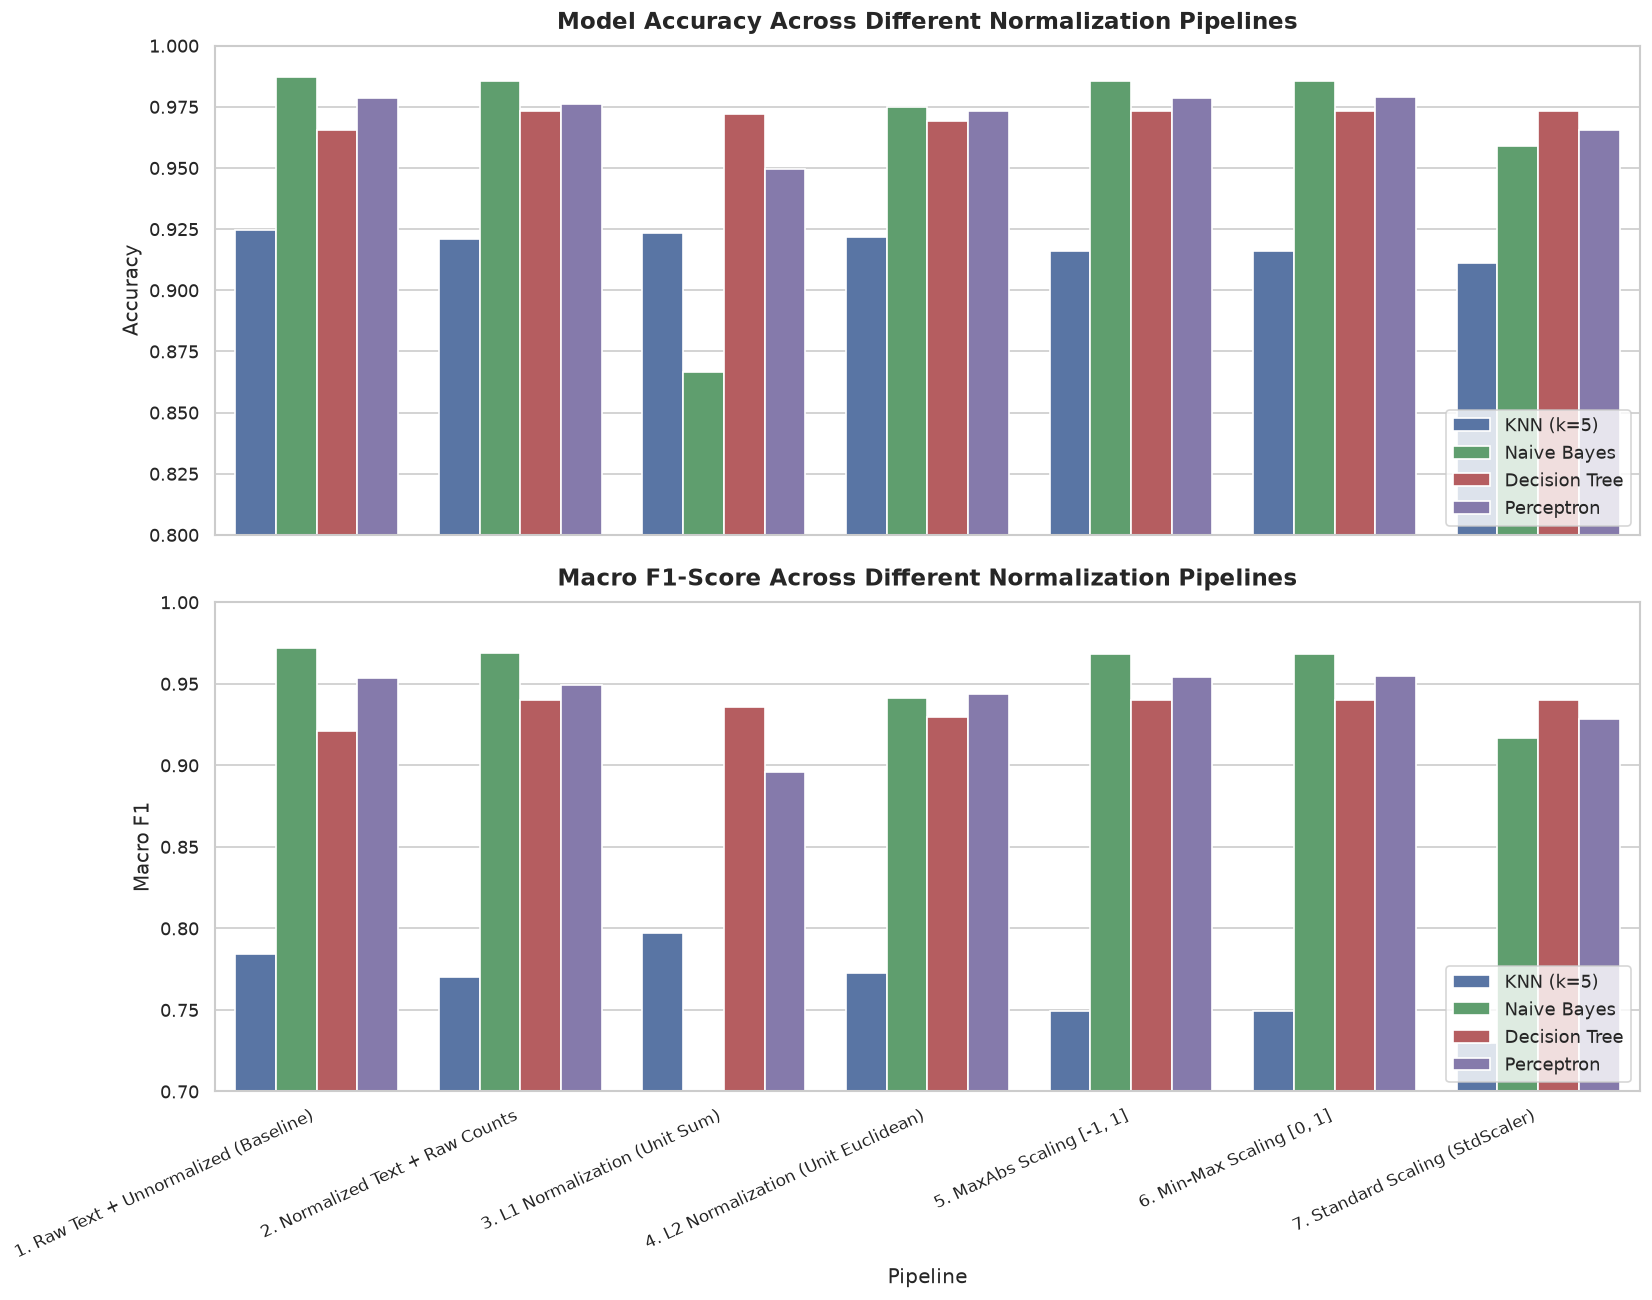
\includegraphics[width=0.98\textwidth]{figures/accuracy_macro_f1_bars.png}
    \caption{Comparative grouped bar charts depicting Model Accuracy (top) and Macro F1-Score (bottom) across all seven normalization pipelines.}
    \label{fig:accuracy_f1_bars}
\end{figure}

\subsection{Performance Delta Heatmap}
To isolate the precise gain or penalty attributable to each normalization method, Figure~\ref{fig:delta_heatmap} presents the percentage point delta ($\Delta \text{Accuracy} = \text{Accuracy}_{\text{pipeline}} - \text{Accuracy}_{\text{baseline}}$).

\begin{figure}[H]
    \centering
    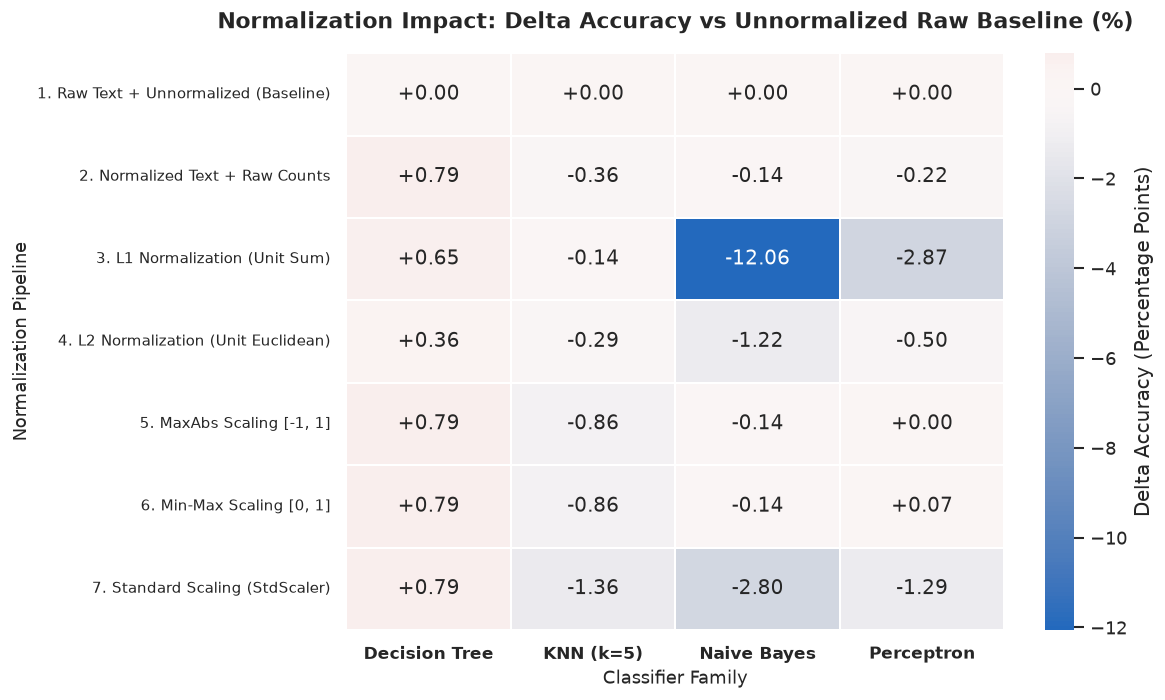
\includegraphics[width=0.78\textwidth]{figures/normalization_delta_heatmap.png}
    \caption{Performance Delta Heatmap illustrating the percentage point difference in accuracy relative to the unnormalized raw baseline. Positive values (red) denote performance gains, while negative values (blue) denote degradation.}
    \label{fig:delta_heatmap}
\end{figure}

\subsection{Confusion Matrix Contrasts}
Figure~\ref{fig:confusion_matrices} provides an 8-panel diagnostic contrast comparing baseline raw text counts against optimal $L_2$ Euclidean normalization.

\begin{figure}[H]
    \centering
    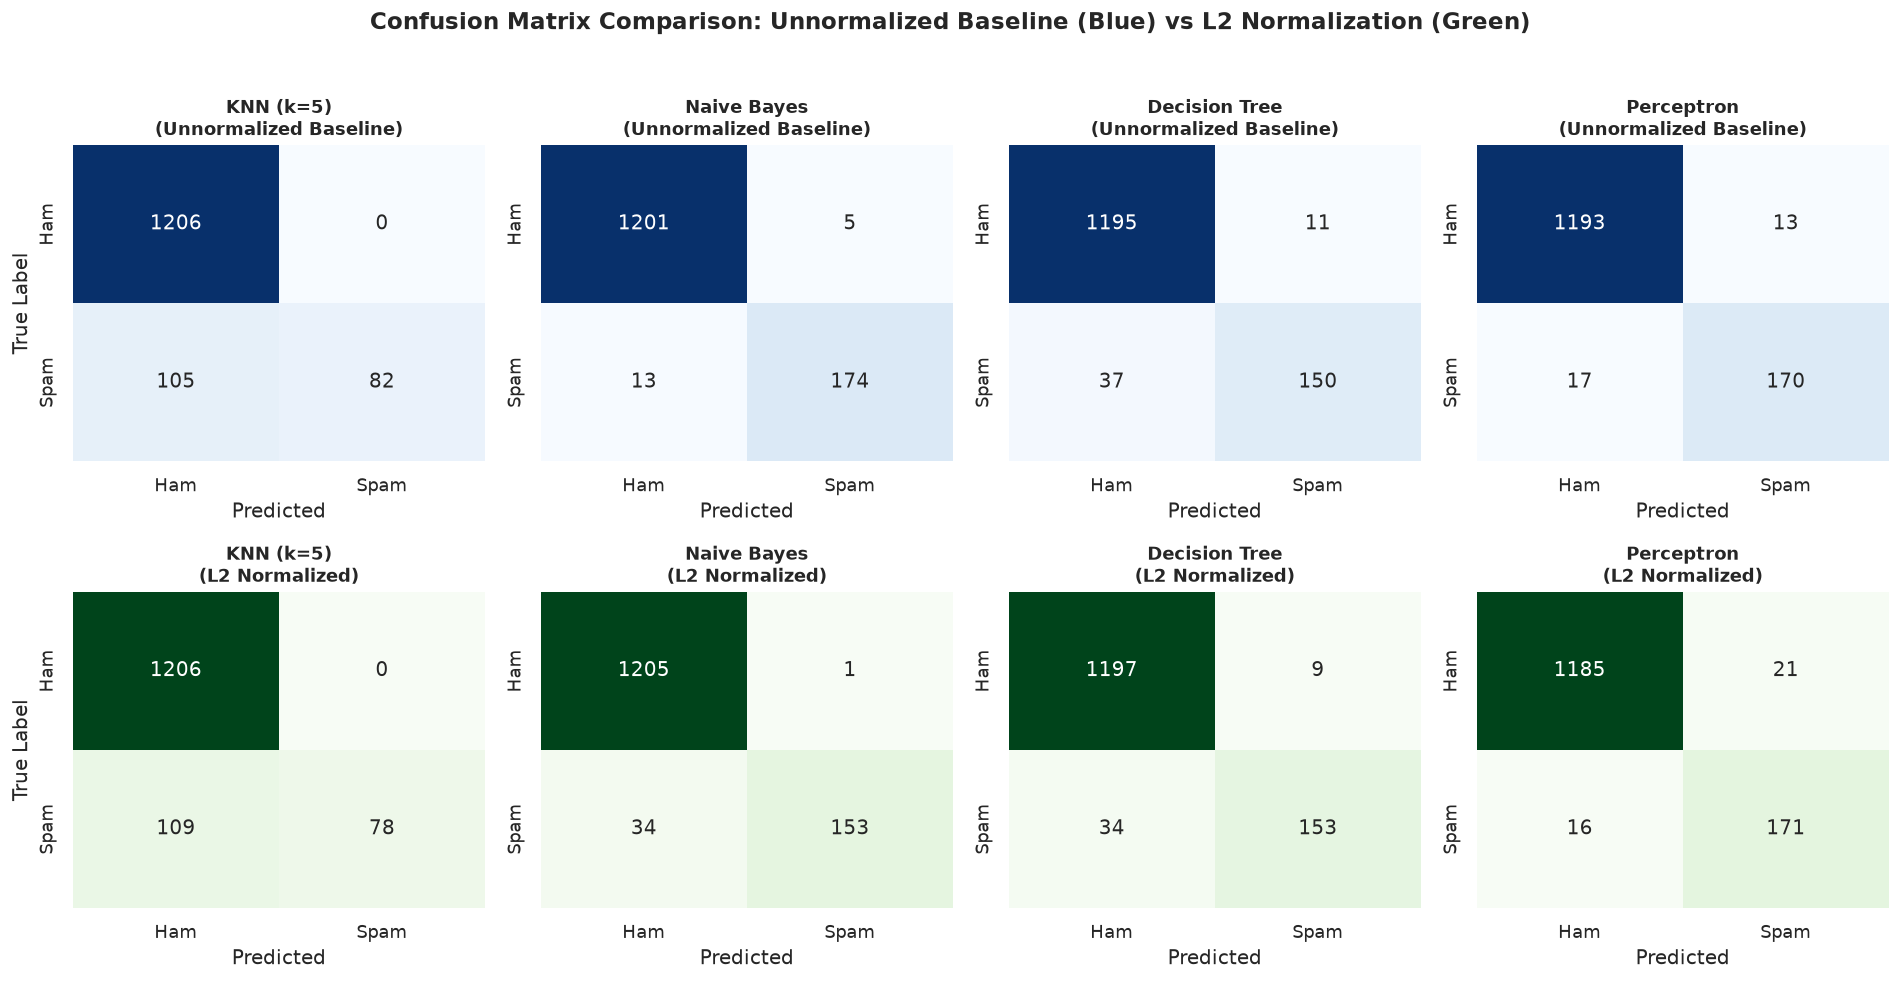
\includegraphics[width=0.98\textwidth]{figures/confusion_matrices_comparison.png}
    \caption{Multi-model confusion matrix comparison across testing instances ($N=1,393$). Top row: Pipeline 1 (Raw Text Baseline); Bottom row: Pipeline 4 ($L_2$ Euclidean Normalization).}
    \label{fig:confusion_matrices}
\end{figure}

\newpage
\section{In-Depth Theoretical Discussion: Classifier Sensitivities}

The empirical benchmarks reveal starkly divergent responses to normalization across the four classifier families:

\subsection{1. K-Nearest Neighbors (KNN)}
\begin{itemize}
    \item \textbf{Mathematical Vulnerability}: In raw unnormalized text, message length directly distorts Euclidean distance:
    \begin{equation}
        d(\mathbf{u}, \mathbf{v}) = \sqrt{\sum_{j=1}^{D} (u_j - v_j)^2}
    \end{equation}
    A long message containing benign filler words generates large coordinates, placing it artificially distant from semantically identical short messages.
    \item \textbf{Resolution via $L_2$ Normalization}: Projecting vectors onto the unit sphere ($\|\mathbf{u}\| = 1$) makes Euclidean distance an exact linear transform of Cosine Similarity ($d^2 = 2 - 2\cos\theta$). This stabilizes neighborhoods and mitigates document length bias.
\end{itemize}

\subsection{2. Naive Bayes (MultinomialNB / ComplementNB)}
\begin{itemize}
    \item \textbf{The $L_1$ Collapse}: Multinomial Naive Bayes computes posterior class probabilities via:
    \begin{equation}
        P(c \mid \mathbf{x}) \propto P(c) \prod_{j=1}^{D} P(w_j \mid c)^{x_j}
    \end{equation}
    When integer word counts ($x_j \ge 1$) are converted into tiny fractional sums via $L_1$ normalization ($\sum x_j = 1.0 \implies x_j \approx 0.02$), the exponents shrink towards zero ($P(w_j \mid c)^{0.02} \approx 1.0$), severely flattening the likelihood ratio. Consequently, Naive Bayes accuracy plummeted from $98.71\%$ down to $86.65\%$, and Macro F1 collapsed to $0.4695$ (predicting almost exclusively the majority \texttt{ham} class).
    \item \textbf{Standard Scaling Incompatibility}: Standard scaling subtracts column means, introducing negative entries ($z_{i,j} < 0$) which are mathematically undefined as multinomial word occurrences.
\end{itemize}

\subsection{3. Decision Tree Classifier}
\begin{itemize}
    \item \textbf{Strict Monotonic Scale Invariance}: At every internal node, decision trees evaluate threshold conditions $x_j \le \theta$. For any strictly monotonic 1D coordinate scaling (such as Min-Max or MaxAbs):
    \begin{equation}
        x_a < x_b \iff f(x_a) < f(x_b)
    \end{equation}
    Sample ranking is perfectly preserved, rendering optimal split locations identical. Table~\ref{tab:accuracy_results} proves that Min-Max, MaxAbs, and Standard Scaling yielded identical accuracy ($97.34\%$) and Macro F1 ($0.9400$).
    \item \textbf{Vector-Wise Alteration}: $L_1$ and $L_2$ normalizations divide $x_{i,j}$ by document-level sums $\sum_k x_{i,k}$, introducing cross-feature coupling that alters sample ranks along individual axes, allowing the tree to find altered splits ($97.20\%$ and $96.91\%$).
\end{itemize}

\subsection{4. Perceptron (Linear Hyperplane)}
\begin{itemize}
    \item \textbf{Gradient Step Stabilization}: Perceptron updates satisfy $\Delta \mathbf{w} = \eta (y_i - \hat{y}_i) \mathbf{x}_i$. Unbounded raw counts cause volatile parameter oscillations when long messages are misclassified. Restricting input norms via Min-Max or MaxAbs scaling stabilizes the step size, elevating accuracy to $97.92\%$.
\end{itemize}

\subsection{Production NLP Normalization Decision Matrix}
Table~\ref{tab:decision_matrix} provides architectural engineering guidelines synthesized from this empirical investigation.

\begin{table}[H]
\centering
\caption{Practical Normalization Decision Matrix in Applied Machine Learning / NLP}
\label{tab:decision_matrix}
\vspace{0.2cm}
\begin{tabular}{p{3.5cm}p{4.0cm}p{3.8cm}p{3.5cm}}
\toprule
\textbf{Model Family} & \textbf{Primary Sensitivity} & \textbf{Recommended Normalization} & \textbf{Normalization to Avoid} \\
\midrule
\textbf{KNN / Metric-Based} & Extreme (Distance distorted by document length) & \textbf{$L_2$ Normalization / Cosine Metric} & Raw unnormalized counts \\
\addlinespace
\textbf{Naive Bayes (Multinomial)} & Severe (Requires non-negative frequency weights) & \textbf{Raw Counts, TF-IDF, or MaxAbs} & $L_1$ normalization, negative $Z$-scores \\
\addlinespace
\textbf{Decision Trees / Ensembles} & None (Monotonically invariant to 1D scaling) & \textbf{Raw Cleaned Counts or $L_2$} & Dense scalers (wastes memory) \\
\addlinespace
\textbf{Linear Models (Perceptron, SVM)} & High (Step size proportional to input norm $\|\mathbf{x}\|$) & \textbf{Min-Max, MaxAbs, or $L_2$} & Unbounded raw counts \\
\bottomrule
\end{tabular}
\end{table}

\section{Conclusion}
In this laboratory assignment, the mathematical foundations and empirical implications of text-level and feature-level normalization were investigated on the SMS Spam Collection corpus.
\begin{itemize}
    \item \textbf{Best Performing Architecture}: Multinomial Naive Bayes trained on raw unnormalized BoW features achieved the highest overall accuracy ($98.71\%$) and Macro F1 ($0.9717$).
    \item \textbf{Harmful Normalization}: $L_1$ normalization catastrophic collapsed Naive Bayes performance ($46.95\%$ Macro F1) by flattening term occurrence exponents.
    \item \textbf{Essential Normalization}: $L_2$ Euclidean normalization proved essential for distance-based metric models (KNN) by projecting documents onto the unit hypersphere, neutralizing message length bias.
    \item \textbf{Scale Invariance}: Decision Trees confirmed theoretical expectations of strict scale invariance under monotonic coordinate transformations.
\end{itemize}

\end{document}

